% $Id: jmldbc.tex,v 1.40 2006/11/13 18:39:06 leavens Exp $

\documentclass[twocolumn]{article}
\usepackage{hyperref}
\usepackage{url}
\usepackage[dvips]{graphicx}
\usepackage{verbatim}
\setlength{\textheight}{9in}
\setlength{\headheight}{.60in}
\setlength{\headsep}{.40in}
\setlength{\topmargin}{-1in}


\setlength{\textwidth}{6.5in} 
\setlength{\oddsidemargin}{0in}		% i.e. 1 inch margins
\setlength{\evensidemargin}{0in}




\def\RESULT{\texttt{\char'134result}}
\def\OLD#1{\texttt{\char'134old({#1})}}

\title{Design by Contract with JML}
\author{
  \begin{tabular}{ccc}
  Gary T. Leavens          & \hspace{0.2in} & Yoonsik Cheon\\~\\
  Dept. of Computer Science && Dept. of Computer Science\\
  Iowa State University    && University of Texas at El Paso\\
  Ames, IA 50010           && El Paso, TX 79968\\
  \texttt{leavens@cs.iastate.edu} && \texttt{cheon@cs.utep.edu}
  \end{tabular}
}

\date{September 28, 2006}

\begin{document}

\maketitle

\begin{abstract}
  This document gives a tutorial introduction to the Java Modeling
  Language (JML), and explains how JML can be used as a powerful design by
  contract (DBC) tool for Java. JML is a formal behavioral interface
  specification language for Java that contains the essential
  notations used in DBC as a subset.  The basic concepts of DBC are
  explained with a particular emphasis on how to use JML notations to specify
  Java classes and interfaces.  JML tools such as JML compiler
  (\texttt{jmlc}) are also introduced, with examples of their use.
\end{abstract}

\section{Motivation}
\subsection{Design by Contract}

\emph{Design by contract} (DBC) is a method for developing software
\cite{Meyer92a}.  
The principal idea behind DBC is that a class and its clients have a
``contract'' with each other. The client must guarantee certain
conditions before calling a method defined by the class, and in return
the class guarantees certain properties that will hold after the call.
The use of such pre- and postconditions to specify software dates back
to Hoare's 1969 paper on formal verification \cite{Hoare69}.
What is novel about DBC is that it makes these contracts
executable.  The contracts are defined 
by program code in the programming language itself, and are translated
into executable code by the compiler.  Thus, any violation of the
contract that occurs while the program is running can be detected immediately.

A contract in software specifies both obligations and rights of
clients and implementors.
For example, a contract for a method, \texttt{sqrt}
that takes a number and returns its square root may be specified as in
Figure~\ref{fig:prepost}.
(The static method \texttt{approximatelyEqualTo} of the class
\texttt{JMLDouble} tests whether the relative difference of 
the first two double arguments is within the given epsilon,
the third argument.)

\begin{figure}
\begin{verbatim}
 //@ requires x >= 0.0;
 /*@ ensures JMLDouble
   @         .approximatelyEqualTo
   @          (x, \result * \result, eps);
   @*/
 public static double sqrt(double x) {
   /*...*/
 }
\end{verbatim}
\caption{Pre- and postconditions in JML (lines 1-4) for the method
  \texttt{sqrt}}
\label{fig:prepost}
\end{figure}

JML specifications are written in special \emph{annotation
comments\/}, which start with an at-sign (\texttt{@}).
At-signs at the beginnings of lines in annotation comments of the form
\texttt{/*@ ... @*/} are ignored.
Note that the at-sign, \texttt{@}, must be right next to the start of
comment characters.  A comment starting \texttt{//~@} will be ignored
by JML, whereas \texttt{//@} starts an annotation properly.
Similarly, \texttt{/*~@} will not start an annotation, instead one
must use \texttt{/*@}.  (JML tools do not currently warn about comments that
might use such mistaken annotation markers.)

JML uses a \texttt{requires} clause to specify the
client's obligation and an \texttt{ensures} clause to specify the
implementor's obligation.  The obligation of the client in this case is
to pass a positive number as an argument (\texttt{x}). On the other
hand, the client has the right to get a square root approximation as
the result ({\verb|\result|}). Similarly, the implementor can assume
that the argument is a positive number, but has an obligation to
compute and return a square root approximation.

% pre and postconditions

As in the previous example,
a contract is typically written by specifying a method's pre and
postconditions.  A method's \emph{precondition} says what must be true
to call it. The precondition of our square root method may be
specified as follows. (JML uses the keyword \texttt{requires} to introduce
a precondition.)

\begin{verbatim}
  //@ requires x >= 0.0;
\end{verbatim}

A method's \emph{postcondition} says what must be true when it terminates.
In a language like Java that supports exceptions, we further
distinguish normal and exceptional postconditions.
A method's \emph{normal postcondition} says what must be true when it
returns normally, i.e., without throwing an exception. For example,
the normal postcondition of our square root method may be specified as
follows. (JML uses the keyword \texttt{ensures} to introduce a
normal postcondition.)

\begin{verbatim}
 /*@ ensures JMLDouble
   @         .approximatelyEqualTo
   @          (x, \result * \result, eps);
   @*/
\end{verbatim}

(JML allows the specification of what exceptions a method may throw as
well.  This can be done using JML's \verb|signals_only| clause.
However, the default for the \verb|signals_only| clause is to only
allow exceptions named in the method header's \texttt{throws} clause.
Since in Figure~\ref{fig:prepost} no \texttt{throws} clause appears in
the method header, the method has a default \verb|signals_only| clause
that prohibits exceptions from being thrown, when the precondition
holds.  Thus, beginning JML users can usually ignore the
\verb|signals_only| clause, and the \texttt{signals} clause, which
allows one to specify more details about the program state when
exceptions are thrown.
Instead, when learning JML, one should concentrate on specifying
preconditions that are strong enough to rule out exceptional
behaviors.)

In JML specifications are typically written just before the header
of the method they specify.  An example is given in
Figure~\ref{fig-SqrtExample}.  The \texttt{sqrt} method given in this
figure is intended for trusted users. It assumes that the
argument is positive, and in this case returns the necessary
approximation.  If the argument is negative, and if the code has been
compiled with the JML runtime assertion checking compiler, then the
call will result in a runtime error, due to the violation of the specified
precondition. 

\begin{figure*}
\verbatiminput{samples/SqrtExample.java}
\caption{The file SqrtExample.java}
\label{fig-SqrtExample}
\end{figure*}

% relational model of methods
%% [[[Should we omit the following?]]]
% The origin of DBC is formal specification and verification of
% programs, in particular Hoare logic \cite{Hoare69}.
% Using Hoare logic, one can prove
% the correctness of a program with respect to a formal specification.
% One way of specifying programs is to view them as defining relations
% between inputs and outputs.  For example, a method can be viewed as
% defining a relation between arguments and results.  In this viewpoint,
% the precondition describes the domain of the relation and the
% postcondition describes the relationship itself.

In summary, DBC is a way of recording details of method
responsibilities. It can be used for internally called methods to 
avoid constantly rechecking the validity of arguments.
It can also be used to specify the effect of calling a method, and
thus for recording details in a design.
Some of these aspects will be further explained in the following
subsections as we explain more about JML.

\subsection{Documentation}

Using DBC provides good documentation for program modules such as Java
classes and interfaces. For each method of a class or interface, the contract
says what it requires, if anything, from the client and what it
ensures to the client, as in the examples above and in
Figure~\ref{fig-SqrtExample}. 

DBC is better for documentation than just code;
and is even better than using informal documentation, such as program
comments or Javadoc comments.
A DBC contract specification is more abstract than code; in part this
is because it doesn't have to give an algorithm in detail, but can
concentrate on what is assumed and what must be achieved.
Unlike comments, a formal specification in JML is (usually)
machine checkable, and so can help with debugging.
That is, checking the specification can help isolate errors before
they propagate too far.
In addition, because a JML specification is checked mechanically, it
has a much greater chance of being kept up-to-date with respect to the
code than informal documentation.

% abstraction by specification

How is constructing a square root different than the specification of
the \texttt{sqrt} method in Figure~\ref{fig-SqrtExample}?
The main difference is that the contract given in the specification
can be satisfied in many different ways. 
For example, the square root method \texttt{sqrt} may be implemented
by calling a library routine (as shown), calling another method
written by the user, or directly by using linear search, binary
search, Newton's method, etc.  These will have varying non-functional
properties such as efficiency and memory usage.  However, the
specification abstracts from all these 
implementation details. This means that the implementation can
be changed later without invalidating the client code as long as the new
implementation still satisfies the contract.  For example, in
\texttt{sqrt}, the call to \texttt{Math.sqrt} could be replaced
with another algorithm to compute square roots, and clients would not be
affected. In summary, a contract
is an abstraction of a method's behavior.
While in many cases the contract is about the same length as the code
(as shown in Figure~\ref{fig-SqrtExample}),
in some cases it can be considerably shorter (for example, if the code
for computing square roots by Newton's method were written in the body
of \texttt{sqrt}).

\subsection{Blame Assignment}

Another advantage of DBC is that it can be used to assign
blame to a faulty part of a program.  For example, who is to be
blamed if \texttt{sqrt}'s precondition doesn't hold?  Clearly this
isn't the fault of \texttt{sqrt}, which hasn't even started to run
yet, so the fault must lie with the caller.
Thus, the client code, the code that calls \texttt{sqrt} has to be fixed.

Similarly, who is to be blamed if, at the end of processing of a
call to \texttt{sqrt} in which its precondition held,
it turned out that \texttt{sqrt}'s postcondition didn't hold?
The code of \texttt{sqrt} (and the methods it calls)
must contain the fault, because the implementor has broken
their side of the contract. Thus, the implementing code, in
\texttt{sqrt} and the methods it calls, has to be fixed.

\subsection{Efficiency}

DBC also allows one to avoid inefficient defensive checks, which can
otherwise cripple the efficiency of code.
For example, the \texttt{sqrt} method in
Figure~\ref{fig-SqrtExample} assumes that its argument is
non-negative.  This trust is validated by checking the
preconditions during debugging, but these checks can be turned off for
production use of the program.

Another aspect of efficiency is that defensive checks are sometimes
not possible to execute efficiently.  For example, consider the
example below, in which a binary search method requires that its array
argument be sorted.  Checking that an array is sorted requires time
linear in the length of the array, but the binary search routine is
supposed to execute a logarithmic time.  Therefore the defensive
checks would slow down the method unacceptably.  In this example,
contracts, which are easier to automatically remove when the program
goes into production, are much more efficient.

\begin{verbatim}
  /*@ requires a != null 
    @       && (\forall int i;
    @               0 < i && i < a.length;
    @               a[i-1] <= a[i]);
    @*/
  int binarySearch(int[] a, int x) {
    // ... 
  }
\end{verbatim}

In the above, the precondition of \texttt{binarySearch} says that the
array cannot be null, and that for all integers \texttt{i},
if \texttt{i} is strictly greater than 0 and strictly less than the
length of the array argument \texttt{a}, then the element
\texttt{a[i-1]} is no larger than \texttt{a[i]}.
Note that this universally quantified expression in JML must have
parentheses around it, \verb|(\forall| $\dots$\verb|)|.
In some sense it is a bit like a \texttt{for}-loop in Java, with a
declaration (but no initialization), a predicate that describes the
range of the declared variable, and a body.  However the body is not a
statement but a Boolean-valued expression; the body must be true for
all of the values of the variable that fall in the described range for the
\verb|(\forall| $\dots$\verb|)| expression to be true.  (The range is
optional, but if omitted, such a universally quantified expression may
not be executable; it can still be used for documentation purposes, however.)

\subsection{Modularity of Reasoning}

Another important benefit of DBC is that it supports modularity of
reasoning.
As an example, consider the following typical object-oriented code.

\begin{verbatim}
  ...
  source.close();
  dest.close();
  getFile().setLastModified(
    loc.modTime().getTime());
  return modTime();
\end{verbatim}

How can we understand this code?  There are
two ways. We could read either the code for all the methods or the
contracts for all the methods.
However, if you try to read the code for all the methods the same
problem occurs again --- how do you understand that code?
If the program is small you will run out of code to read, but in code
that is from a large program, or that makes heavy use of method calls, and
especially one in which there is much use of subtype polymorphism
(dynamic binding), it can be very difficult to understand what is
going on in a reasonable amount of time.
If you have had experience of reading object-oriented source code
(especially written by others or by yourself written quite a long time
ago), you will have encountered this problem.  That is, you will have
seen the problem of non-modular reasoning.  Reasoning is
\emph{non-modular\/} if to reason about one piece of code, you have to
reason about many other pieces of code.

A better way is to read the specifications of the other methods.
If the specifications are appropriately abstract, you do not have to
keep reading many more specifications to understand what a method call
does; the process bottoms out more quickly.  In any case, you did not
need to read other code, so the process is, by definition, \emph{modular}.

\subsection{The Cost of Modularity}

In return for the benefit of faster understanding, modular reasoning
imposes a cost.  This cost is that clients are not allowed to conclude
anything that is not justified by the contracts of the methods that
they call.  Another way of looking at this is that,
to allow modular reasoning with contract specifications, the
client code must work for every implementation that satisfies
the contract.  Thus reasoning about client code can only use the
contracts (not the code!) of methods that are called.
In addition, clients are obligated to establish the precondition of
each method called.  But in return they are saved the trouble of
achieving the postcondition themselves.  Consider the following
example.  (In this example, we use two JML assert statements around a
piece of Java code.)  In this example, we can conclude that the result
of the call is approximately 3.0.

\begin{verbatim}
  //@ assert 9.0 >= 0.0;
  double res = SqrtExample.sqrt(9.0);
  /*@ assert JMLDouble
    @        .approximatelyEqualTo
    @         (9.0, res * res,
    @          SqrtExample.eps);
    @*/
\end{verbatim}

What is not permitted in this example is to look at the code for the
\texttt{sqrt} method, see that it calls \texttt{Math.sqrt}, and conclude from
this that the result is accurate to, say, 7 decimal places.  The
contract only specifies that the result is an approximation that is
correct to 4 decimal places (which is the value of \texttt{SqrtExample.eps}).
But if the method is actually computing
the square root with an accuracy of 7 decimal places, what is wrong
with using this extra information?  The problem is that doing so would
tie the client to the actual implementation of the method as opposed
to the contract.  In other words, the implementation would no longer
be free to change the algorithm used to compute square roots.
For example, the algorithm could not be changed to be a faster one
that only computed square roots to 4 decimal places of accuracy.
In summary, client code must only reason about the specifications of
the methods it calls, not their code.

\subsection{Contracts and Intent}

There are other good reasons not to use code as contracts. Code makes a poor
contract, because by only using code one cannot convey to readers
what is intended (i.e., what the essential properties of the method
are) and what parts are merely implementation decisions (accidental
features).  For example, if the code for \texttt{sqrt} computes square
roots to 7 decimal places, cannot this be changed in the next release?
Without some separate description of what is intended,
the reader can't tell if that 7 decimal places were intended, or just
happened to be computed; perhaps 4 decimal places are all that is
necessary for the rest of the program.
By contrast, contracts allow implementors to specify their
intent and freedom to change inessential details. Thus contracts tell
clients what they can count on and what is essential, while leaving
implementors the freedom to change inessential details, for example
to make code run faster.

Here is a question for you. What kinds of changes might vendors want
to make that don't break existing contracts?

\section{What is JML?}

JML stands for ``Java Modeling Language''.  It is a formal behavioral
interface specification language for Java.
As such it allows one to specify both the syntactic interface of
Java code and its behavior.  The \emph{syntactic interface\/} of Java code
consists of names, visibility and other modifiers,
and type checking information.
For example, the syntactic interface of a method can be seen in the
method's header, which lists its modifiers, name, return
type, the types of its formal parameters, and the types of the
(checked) exceptions it may throw.
The \emph{behavior\/} of Java code describes what should happen at
runtime when the code is used.  For example the behavior of a method
describes what should happen when the method is called;
as we have discussed above, the behavior of a method is often
specified using pre- and post conditions.
Since JML can document both the syntactic interface and behavior of
Java code, it is well-suited to documenting detailed design decisions
about Java code \cite{Leavens-Baker-Ruby06}.

JML combines the practicality of DBC language like Eiffel
\cite{Meyer92b} with the expressiveness and formality of
model-oriented specification languages.  As in Eiffel, JML uses Java's
expression syntax to write the predicates used in \emph{assertions},
such as pre- and postconditions and invariants.
The advantage of using Java's notation in assertions
is that it is easier for programmers to learn and less
intimidating than languages that use special-purpose mathematical
notations. However, Java expressions lack some expressiveness
that makes more specialized assertion languages convenient for writing
behavioral specifications.
JML solves this problem by extending Java's expressions with various
specification constructs, such as quantifiers.

JML is unique in that it is designed to be used with a wide range of
tools \cite{Burdy-etal05,Leavens-etal05}.
These tools support DBC, runtime assertion checking, discovery of
invariants, static checking, specification browsing, and even
formal verification using theorem provers.
These support tools are freely available from the JML web page
\url{http://www.jmlspecs.org} 
(see Appendix~\ref{sect-appendix} for downloading and installing JML
tools).
For example, JML incorporates many ideas and concepts from
model-oriented specification languages,
which allows one to write specifications that are suitable for formal
verification.  The benefit of JML's design is that such features are
also useful with other tools, as they help make specifications more
abstract and succinct.
However, novice users need not fear all of these features;
as we show in this document, JML has a small subset that can be used
as a DBC language for Java.  

\section{Simple Examples}
\subsection{Informal Specifications}

The first step to writing contracts is to organize program comments
that describe methods as contracts.
That is, one should organize the comments about a method's behavior
into preconditions and postconditions.
JML supports this without requiring that these comments be formalized
by allowing informal descriptions in specifications.
An \emph{informal description} looks like the following:

\begin{verbatim}
  (* some text describing a property *)
\end{verbatim}

JML treats an informal description as a boolean expression.
This allows informal descriptions to be combined with formal
statements, and is convenient when the formal statement is not easier
to write down or clearer.
For example, the following JML specification describes the behavior of
the method \texttt{sqrt} using informal descriptions.

\begin{verbatim}
  //@ requires (* x is positive *);
  /*@ ensures (* \result is an
    @            approximation to
    @            the square root of x *)
    @      && \result >= 0;
    @*/
  public static double sqrt(double x) {
    return Math.sqrt(x);
  }
\end{verbatim}

As an exercise, write informal pre and postconditions for the other
methods of the class \texttt{Person} shown in
Figure~\ref{fig-write-informal-spec}. Are the informal specifications
longer than the code sometimes?

\begin{figure}
\verbatiminput{samples/Person.java}
\caption{A class \texttt{Person} to be filled with informal specifications.
  The keyword \texttt{also} in the specification of the method
  \texttt{toString} indicates that the method ``also'' inherits
  specifications from its supertypes (i.e., the class \texttt{Object}
  in this case).}
\label{fig-write-informal-spec}
\end{figure}

Informal specifications are convenient for organizing informal
documentation.  Informal specifications can also be very useful when
there's not enough time to develop a formal description of some aspect
of the program.  For example, currently JML does not have a formal
specification for input and output.  Thus, methods that write to and read
from files typically have to use informal descriptions to describe
parts of their behavior.  This kind of escape from formality is very
useful, in general, to avoid describing the entire world formally when
writing a specification of some method.

However, there are several drawbacks to using informal descriptions.
A major drawback is that informal descriptions are often ambiguous or
incomplete.  Another problem is that informal descriptions cannot be
manipulated by tools.  For example, JML's runtime assertion checker
has no way of evaluating informal descriptions, so these cannot be
checked at runtime.  Thus, whenever time permits, one should try to
use formal notation instead of informal descriptions.

\subsection{Formalization}
\label{sect-formalization}

Figure~\ref{fig-formal-spec} shows the class \texttt{Person} of the
previous section with all its methods formally specified in JML.
Formal specifications in JML are written using an extended form of
Java expressions.  Specification expressions in JML also have some
restrictions, compared to Java.

\subsubsection{JML Specification Expressions}

Some of the extensions JML adds to Java expressions
are shown in Table~\ref{tbl-jml-extension}.
These include a notation for describing the result of a method
(\RESULT), various kinds of implication\footnote{In addition, JML
also support various forms of quantifiers
(see Section~\ref{sect-quantifiers}).},
and a way of referring to the pre-state value of an expression
(\OLD{$\cdot$}).
We have seen the use of {\RESULT} already, for example in
Figure~\ref{fig-SqrtExample}.
An example of the use of \OLD{$\cdot$} appears in the specification of
the \texttt{addKgs} method of the class \texttt{Person} in
Figure~\ref{fig-formal-spec}.  In the normal postcondition,
the expression 
``\texttt{weight == \OLD{weight + kgs}}''
is true when the value of \texttt{weight} at the end of the method
(just before it returns to its caller), is equal to the value the expression
``\texttt{weight + kgs}'' had at the beginning of the method call
(just after parameter passing).

\begin{table}
\caption{Some of JML's extension to Java expressions}
\label{tbl-jml-extension}
\begin{center}
\begin{tabular}{|l|l|}\hline
  Syntax& Meaning\\\hline\hline
  {\RESULT} & result of method call\\
  \texttt{$a$ ==> $b$} & $a$ implies $b$\\
  \texttt{$a$ <== $b$} & $a$ follows from $b$ (i.e., $b$ implies $a$) \\
  \texttt{$a$ <==> $b$} & $a$ if and only if $b$\\
  \texttt{$a$ <=!=> $b$} & not ($a$ if and only if $b$)\\
  \OLD{$E$} & value of $E$ in pre-state\\\hline
\end{tabular}
\end{center}
\end{table}

% moved here so will fall on a different page than {fig-write-informal-spec}
\begin{figure}
\verbatiminput{samples/Person.refines-java}
\caption{Class \texttt{Person} with formal specifications.  This
  specification would appear in a file named \texttt{Person.refines-java}.}
\label{fig-formal-spec}
\end{figure}

The main restriction in JML is that expressions used in JML's
assertions cannot have side effects. Thus Java's assignment
expressions (\texttt{=}, \texttt{+=}, etc.) and its increment
(\texttt{++}) and decrement (\texttt{--}) operators are not
allowed. In addition, only pure methods can be called in assertions.
A method is \emph{pure} if it has no side-effects on the program's
state. Some authors call such methods ``query'' methods, because they
can be used to ask about the state of an object without changing it.
One must tell JML that a method to be pure by using the
\texttt{pure} modifier in the method's declaration.
For example, the \texttt{getWeight} method in
Figure~\ref{fig-formal-spec} is declared to be \texttt{pure}.
It could thus be called in an assertion; for example a client might
specify that the weight of a person \texttt{p} be not too high by writing
\texttt{p.getWeight < 200}.
Methods that are not declared to be pure are assumed not to be pure,
and cannot be used in specification expressions.

\subsubsection{Information Hiding in Specifications}

JML supports the notion of information hiding by using
Java's privacy levels.
In the DBC style of JML usage that we are describing in this document,
the privacy of a method or constructor specification is the
same as that of the method or constructor it specifies.\footnote{
Privacy can be explicitly specified in the
heavyweight form of JML method and constructor specifications
\cite{Leavens-Baker-Ruby06}.}
For example, all the method specifications in Figure~\ref{fig-formal-spec}
have public visibility, because they annotate public methods.
The invariant in Figure~\ref{fig-formal-spec} is also
publicly-visible, however its visibility is explicitly specified by using
the modifier \texttt{public}; without that modifier it would only be
visible to clients in the same package.

JML enforces information hiding by ensuring that public specifications
can only mention publicly-visible names.
That is, JML does not allow private fields to be used in public
specifications. 
Thus, for example, since the method, constructor, and invariant
specifications in Figure~\ref{fig-formal-spec} all have public
visibility, they can only mention publicly-visible names.  This is the
reason for the annotation ``\texttt{spec\_public}''
in the declaration of the fields \texttt{name} and \texttt{weight}.
This annotation says that \texttt{Person}'s fields \texttt{name} and
\texttt{weight} are to be treated as publicly-visible in JML
specifications, even though Java considers them to be private.

\subsubsection{Non-Null Annotations}

The declaration of the instance field \texttt{name} shows another JML
annotation.  The 
\texttt{non\_null} annotation is a shorthand way of saying that,
in every publicly-visible state, \texttt{name} is not null.
That is, after a constructor returns, and whenever there is no
execution of a method of class \texttt{Person} in progress,
\texttt{name} cannot be null.
(This \texttt{non\_null} annotation is equivalent to the invariant
``\texttt{name != null}''; see Section~\ref{sect-invariants} for details.)

\subsubsection{Underspecification}

A method specification doesn't have to be complete. It is often
intentionally left incomplete, or \emph{underspecified\/} in the sense
that implementations satisfying the specification may have observably
different behaviors.
For example, the specification of the
method \texttt{toString} doesn't exactly specify the return value; all
the specification says is that it is a non-null value.

One reason for using underspecification is to allow implementations to
have more freedom.  In general, this is a good idea, because if you
did not care about some details of the behavior of a method, leaving
it underspecified can allow faster implementations, or implementations
that use less space, or are easier to program.  Underspecification
also allows room for future enhancements.  However, since clients may
only rely on the specification as a contract, it is important to include
in the contract everything that they need to accomplish their work;
that is, everything important about the behavior should be in the contract.

\subsubsection{Semantics}

The meaning of JML method specifications is as follows.  A method must
be called in a state where the method's precondition is satisfied;
otherwise, nothing is guaranteed (the call might loop forever or not
return, or make arbitrary state changes).
The state where a method is called is referred to as a
\emph{pre-state}.  If a method is called in a proper \emph{pre-state},
then there are two possible outcomes of the method's execution.  The
method can return normally or throw an exception.\footnote{
  Other
  possibilities are that the method may either (3) diverge (i.e., loop
  forever or otherwise not return to the caller), or (4) the
  Java Virtual Machine (JVM) may signal an error. JML's
  \texttt{diverges} clause can be used to specify when (3) is allowed.
  Outcome (4) is outside of the control of the programmer, and
  therefore is always allowed. See JML's preliminary design document
  \cite{Leavens-Baker-Ruby06} for details.}
If the method terminates normally without throwing an exception, 
then that termination state is called a \emph{normal post-state}.
If the method terminates by throwing an
exception that does not inherit from the class \texttt{java.lang.Error},
then that termination state is called an
\emph{exceptional post-state}.
In a normal post-state, the method's normal postcondition must be satisfied.
Similarly, in an exceptional post-state,
the exception thrown must be
permitted by the specification's (default or explicit)
\verb|signals_only| clause, and the exceptional post-state must
satisfy the corresponding exceptional postconditions
(\texttt{signals} clauses).

\subsection{Invariants}
\label{sect-invariants}

The specification of the class \texttt{Person} has the following
public invariant clause (see Figure~\ref{fig-formal-spec}).

\begin{verbatim}
  /*@ public invariant !name.equals("")
    @         && weight >= 0;
    @*/
\end{verbatim}

An \emph{invariant\/} is a property that should hold in all
client-visible states.
It must be true when control is not inside the object's
methods.  
That is, an invariant must hold at the end of each constructor's
execution, and at the beginning and end of all methods.\footnote{
  However, in JML, constructors and methods declared with the modifier
  \texttt{helper} are exempted from having to satisfy invariants.
  Such helper methods must be private, and can be used to avoid duplication
  of code, even code that does not start or end in a state that
  satisfies a type's invariants.}

In JML, a public invariant clause allows one to define the acceptable
states of an object that are client-visible;
such invariants are sometimes called \emph{type invariants}.
In JML one can also specify invariants with more restrictive
visibility;
such invariants, which are not visible to clients,
are sometimes called \emph{representation invariants}.
Representation invariants can be used to define acceptable internal
states of an object; for example, that a linked list is circular, or
other similar design decisions.
Public invariants about \texttt{spec\_public}, private fields, such as
this one in \texttt{Person}, have the flavor of both type and
representation invariants. 

As an exercise, formally specify the following method assuming that it
is declared in the class \texttt{Person}.
(Hint: when thinking about the precondition, watch out for the invariant!)

\begin{verbatim}
  public void changeName(String newName) {
       name = newName;
  }
\end{verbatim}

\section{Basic Tool Usage}
\label{sect-tools}

In this section we describe some of the tools that work with JML.

\subsection{Overview of Tools}

Several academic researchers and software contributors have
collaborated on JML, to provide
a range of tools to address the various needs such as
reading, writing, and checking JML specifications \cite{Burdy-etal05}.
The following are the most useful of these for DBC.

\begin{itemize}
\item The JML compiler (\texttt{jmlc}),
is an extension to a Java compiler
and compiles Java programs annotated with JML specifications into Java
bytecode~\cite{Cheon-Leavens02b,Cheon03}.
The compiled bytecode includes
runtime assertion checking instructions that check JML specifications
such as preconditions, normal and exceptional postconditions, and
invariants (see Section~\ref{sect-jml-compiler}).

\item The unit testing tool (\texttt{jmlunit} \cite{Cheon-Leavens02})
combines the JML compiler with JUnit, a popular unit testing tool for
Java~\cite{Beck-Gamma98}. The tool frees the programmer from writing
code that decides test success or failure; instead of writing such
test oracles, the tool uses JML specifications, processed by \texttt{jmlc},
to decide whether the code being tested works properly.

\item The documentation generator (\texttt{jmldoc})
produces HTML containing both Javadoc comments and any JML
specifications.  This makes it possible to browse JML specifications
or to post them on the web.

\item The extended static checker (\texttt{escjava2}),
can find possible mistakes in Java code very quickly.  It is
especially good at finding potential null pointer exceptions and 
array-out-of-bounds indexing operations.  It uses JML annotations to turn off
its warnings and propagates and checks JML specifications.

\item The type checker (\texttt{jml})
is another tool for checking JML specifications, as a faster substitute for
\texttt{jmlc}, if one does not need to compile the code.
\end{itemize}

All the above tools are freely available from the JML web page (refer
to Appendix~\ref{sect-appendix}). 

\subsection{JML Compiler}
\label{sect-jml-compiler}

The JML compiler (\texttt{jmlc}) behaves like Java compilers, such as
\texttt{javac}, by producing Java bytecode from source code file.  The
difference is that it adds assertion checking code to the bytecodes it
produces.  These check JML assertions such as preconditions,
postconditions, and invariants.
The execution of such assertion checking code is
transparent in that, unless an assertion is violated, and except for
performance measures (time and space), the behavior of the original
program is unchanged.  The transparency of runtime assertion checking
is guaranteed, as JML assertions are not allowed to have any
side-effects (see Section~\ref{sect-formalization}).

Using \texttt{jmlc} is similar to using \texttt{javac}.
For example, the following command compiles the file \texttt{Person.java}.
\begin{verbatim}
  jmlc Person.java
\end{verbatim}
This produces a bytecode file, \texttt{Person.class},
in the current working directory.

Sometimes it is convenient to place the output of \texttt{jmlc} in a
directory that is different than that where normal Java compilers put
their output.  To do this, one can use the \texttt{-d} option.
For example, the following command
\begin{verbatim}
  jmlc -d ../bin Person.java
\end{verbatim}
puts the output file, \texttt{Person.class}, it in the directory
\texttt{../bin}. 

By default, \texttt{jmlc} names all the files it is processing.  This
may be reassuring, since \texttt{jmlc} is somewhat slow.  But if one
tires of all this output, one can use the \texttt{-Q} option to
\texttt{jmlc}.  For example, the command
\begin{verbatim}
  jmlc -Q *.java
\end{verbatim}
quietly compiles all the files in the current working directory
whose names end in \texttt{.java}.

For more details on the compilation options available, refer to the
\texttt{jmlc} manual page included in the JML distribution (see
Appendix~\ref{sect-appendix}).
Alternatively, there is a graphical user interface for \texttt{jmlc},
called \texttt{jmlc-gui}, that can be used to run the compiler.  It
makes keeping track of options and selecting files easier.

How to run bytecode compiled with \texttt{jmlc}?  It can be treated as
regular Java bytecode, except that it needs JML's runtime library
classes included in \texttt{jmlruntime.jar} 
to be interpreted by the Java Virtual Machine (i.e., the JVM, which is
the \texttt{java} command). In
particular, the runtime classes must be in the JVM's
``boot class path'';
this is done automatically if you use the script \texttt{jmlrac}.  For
example, given a main program shown in
Figure~\ref{fig-class-personmain}, 
Figure~\ref{fig-class-runpersonmain} is a transcript that
shows how you can compile and run the \texttt{PersonMain} 
and \texttt{Person} classes.
(The output is slightly formatted to fit in this paper's columns.)
This transcript was done on a Linux machine, using the bash shell,
which is reflected in the \verb|$| %$
prompts and the use of the shell variable \verb|$HOME|. %$
The transcript also assumes that the user has installed JML into their
home directory, which is named by \verb|$HOME|, %$ 
so that they have permission to write compiled class files into the
directory containing the samples.

\begin{figure}
\verbatiminput{samples/PersonMain.java}
\caption{Main program to test the class \texttt{Person}}
\label{fig-class-personmain}
\end{figure}

\begin{figure*}
\begin{verbatim}
$ cd $HOME/JML/org/jmlspecs/samples/jmltutorial
$ export CLASSPATH="$HOME/JML"
$ jmlc -Q PersonMain.java Person.java
File "Person.java", line 33, character 12
   warning: The informal description is not executable.
$ jmlrac org.jmlspecs.samples.jmltutorial.PersonMain
Exception in thread "main" 
   org.jmlspecs.jmlrac.runtime.JMLInternalPreconditionError:
   by method Person.Person regarding specifications at
File "Person.refines-java", line 51, character 20 when
  'n' is null
  at org.jmlspecs.samples.jmltutorial.PersonMain.main(PersonMain.java:253)
\end{verbatim}
\caption{Compiling and testing \texttt{PersonMain} and \texttt{Person}.}
\label{fig-class-runpersonmain}
\end{figure*}
%$

If you are using your own Windows machine, you might write the first two
lines as follows, for a typical JML install into \verb|c:\JML|.
\begin{verbatim}
> c:
> cd \
> cd JML\org\jmlspecs\samples\jmltutorial
> set CLASSPATH=c:\JML
\end{verbatim}
The transcript would then continue as in Figure~\ref{fig-class-runpersonmain}.

Do you see why this transcript results in a precondition violation
error?  See the specification of the class \texttt{Person} in
Figure~\ref{fig-formal-spec}.  Note that the line number in the
backtrace (line 253 of \texttt{PersonMain}) does not exist in the
source, as one can tell from Figure~\ref{fig-class-personmain}; this
line number is an artifact of the compilation process.

It is not necessary to compile all the
source files with \texttt{jmlc}.  For example, the driver class
\texttt{PersonMain} may be compiled with a plain Java compiler such as
\texttt{javac}. Only those classes and interfaces that are compiled
with \texttt{jmlc} will be runtime assertion checked.

% [[[I took out the Location example.  Maybe we should have an example that
% we explain better, and it should be integrated with the extra
% features we talk about next.]]]

\section{Other Things in JML}

This section describes a few more advanced features of JML that are
useful in dealing with common problems in specification.

\def\FORALL{\texttt{\char'134forall}}
\def\EXISTS{\texttt{\char'134exists}} 
\def\SUM{\texttt{\char'134sum}}
\def\PRODUCT{\texttt{\char'134product}}
\def\MIN{\texttt{\char'134min}} 
\def\MAX{\texttt{\char'134max}}
\def\NUMOF{\texttt{\char'134num\_of}}

\subsection{Quantifiers}
\label{sect-quantifiers}

JML supports several kinds of quantifiers in assertions: a
\emph{universal quantifier} (\FORALL), an \emph{existential
  quantifier} (\EXISTS), \emph{generalized quantifiers} ({\SUM},
{\PRODUCT}, {\MIN}, and {\MAX}), and a \emph{numeric quantifier}
(\NUMOF).  For example,
the following predicate uses a universal quantifier to assert that all students
found in the set \texttt{juniors} have advisors.

\begin{verbatim}
  (\forall Student s; 
    juniors.contains(s); 
      s.getAdvisor() != null)
\end{verbatim}

In a quantifier, such as the above, there is a declaration,
such as \texttt{Student s}, of a name that is local to the quantifier.
This is followed by an optional range predicate,
such as \texttt{juniors.contains(s)} in the example above;
the range predicate restricts the domain to which the
quantifier applies.
With the range predicate, we quantify over all objects (or values) of
the declared type such that the range predicate is satisfied.
If the range predicate is omitted, there is no restriction on the
objects being quantified over, and so all possible objects apply.
Finally, the third predicate, the body of the quantifier, 
\texttt{s.getAdvisor() != null} in the above example, must be true of
all the objects that satisfy the range predicate.

An equivalent way to write the above example, without an explicit range
predicate, is as follows.

\begin{verbatim}
  (\forall Student s; 
    juniors.contains(s) 
      ==> s.getAdvisor() != null)
\end{verbatim}

The quantifiers {\MAX}, {\MIN}, {\PRODUCT}, and {\SUM}, are
generalized quantifiers that return respectively the maximum, minimum,
product, and sum of the values of their body expression when the quantified
variables satisfy the given range expression.  The numerical
quantifier, {\NUMOF}, returns the number of values for quantified
variables for which the range and the body predicate are true.  For
example, an expression \texttt{({\SUM} int x; 1 <= x \&\& x <= 5; x)}
denotes the sum of values between 1 and 5 inclusive (i.e., 15).

As an exercise, can you write a quantified predicate that asserts that the
elements of an array \texttt{int[] a} are sorted in ascending order? 
Hint: use a nested quantification.
  
\subsection{Inheritance of specifications}

In JML, a subclass inherits specifications such as preconditions,
postconditions, and invariants from its superclasses and interfaces
that it implements.  An interface also inherits specifications of the
interfaces that it extends.
%% [[[Needs work below...]]]
The semantics of specification inheritance
reflects that of code inheritance in Java; e.g., a program variable
appearing in assertions is statically resolved, and an instance method
call is dynamically dispatched.

An important feature of JML's specification inheritance is that its
semantics supports a behavioral notion of subtyping. The essence of
behavioral subtyping is summarized by Liskov and Wing's
\emph{substitution property}, which states that a subtype object can
be used in place of a supertype's object \cite{Liskov-Wing94}.  In
essence, preconditions are disjoined, postconditions are conjoined in
the form of $\bigwedge(\OLD{$p_i$} \Rightarrow q_j)$ (where $p_i$ is a
precondition and $q_j$ is the corresponding postcondition), and
invariants are conjoined.

\subsection{Model Fields}

The class \texttt{Person} in Figure~\ref{fig-formal-spec} was
specified in terms of private, spec\_public fields \texttt{name} and
\texttt{weight}. 
For example, the constructor's postcondition refers to the field
\texttt{name}. But what if you want to change the implementation,
e.g., if you want to use a different data structure?  As a simple
example, consider you want to change a spec\_public field's name from

\begin{verbatim}
  private /*@ spec_public non_null @*/
    String name;
\end{verbatim}

to

\begin{verbatim}
  private /*@ non_null @*/ String fullName;
\end{verbatim}

Ideally, you don't want to make a change to your public specifications
(e.g., the constructor's postcondition), as such a change may affect
the client code because the client relies on the public 
specification.  For specifications, you want to keep the old name
public, but for implementation, you don't want to have two fields
taking up space at runtime.
In JML, you can solve this dilemma by using a model variable.  A
\emph{model variable} is a specification-only variable
\cite{Cheon-etal05}.  For example, you can make the old field a model
field, introduce a new field, and define a relationship between them,
as shown below.

\begin{verbatim}
  //@ public model non_null String name;
  private /*@ non_null @*/ String fullName;
  //@ private represents name <- fullName;
\end{verbatim}

Note that as the new field \texttt{fullName} is private, its existence
is completely hidden from the client. The representation is not
exposed to the client. The \texttt{represents} clause, which is also
private in this case, defines an \emph{abstraction function} that maps
a concrete representation value to an abstract value of the
model field (see Figure~\ref{fig-abstraction-function}).
It says that the value of \texttt{name}
is the same as that of the given expression,
\texttt{fullName} in this case.

In sum, a model variable is a specification-only variable. It is like
a domain-level construct and its value is given by a represents
clause.  In addition to model variables, JML also support model
methods, classes, and interfaces.

Question: how would you modify the specification and implementation to
change the representation of a person's weight from kilograms to
pounds?

\begin{figure}
\centerline{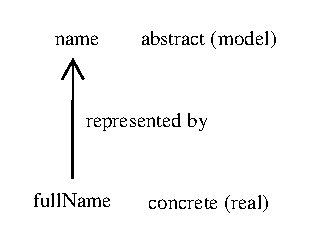
\includegraphics[clip=]{fig-abstraction-function.eps}}
\caption{Mapping concrete values into abstract values.}
\label{fig-abstraction-function}
\end{figure}

\section{Summary}

% [[[Needs work]]]
In this paper we have shown the advantages of DBC and how to use JML
for DBC.

\appendix
\section{Installing JML Tools}
\label{sect-appendix}

JML documentation and tools are freely available from the JML web site
at \url{http://www.jmlspecs.org}. A release of JML is distributed as a
gzipped tar archive file, e.g., \texttt{JML.5.1.tar.gz}.

The installation of JML tools is straightforward. You download the
distribution file and (unzip and) untar it in an appropriate directory
that you want to install JML. Under Microsoft Windows, you can use
WinZip or similar programs to extract it to a directory of your
choice. On Unix, you can use the \texttt{tar} command to extract it.
For example, after saving it to a file
\texttt{/usr/local/JML.5.1.tar.gz}, do the following commands.

\begin{verbatim}
  % cd /usr/local
  % tar -xzvf JML.5.1.tgz
\end{verbatim}

JML tools, documents, sample code, and API specifications will be
extracted into a subdirectory named \texttt{JML}. The subdirectory
\texttt{bin} contains several OS-dependent shell scripts to run
various JML tools, i.e., \texttt{*.bat} files for Microsoft Windows,
\texttt{*-unix} files for Unix, and \texttt{*-cygwin} files for
Cygwin. You need to copy these files to a directory on your
\texttt{PATH} and edit them to change the variable \texttt{JMLDIR} to
the directory where you installed JML.

On Microsoft Windows (e.g., 98, ME, 2000, and XP), copy all
\texttt{.bat} files from \verb|JML\bin| to a directory on your PATH.
Then edit the copied \texttt{.bat} files by changing \texttt{JMLDIR}
to the correct value for you (e.g., \verb|c:\JML|).

On Unix including clones like Linux and Cygwin, use the script
\texttt{bin/Install-JML-Scripts} to install the shell scripts and
manual pages. By default, the shell scripts are installed in the
directory \texttt{/usr/local/bin} and the manual pages in
\texttt{/usr/local/man}. Look and edit the installation script to
install them in other directories and for other options.

For more details on installation, refer to the \texttt{README.html}
file included in the distribution.

\section*{Acknowledgments}

Thanks to students of CS 3331 Advanced Object-Oriented Programming
(Fall 2003 and Spring 2004) at UTEP for comments on earlier drafts of
this tutorial.  Thanks to Francisco Laguna and Faraz Hussain
for comments on an earlier draft.

\bibliographystyle{plain}
\bibliography{jmldbc}

\end{document}
